\subsection{RQ2/RQ3: Security Behaviour and Contribution of the Mechanisms}
\label{sec:ev-sec}

This subsection asks two questions. Does the toolkit that \pamcp{} exposes limit what an injected instruction
could make the agent do? And which of the three mechanisms (G, P, S) is responsible for each measured effect?

\emph{Protocol.} For each of the 155 tasks and each attack class outside the effects the task needs (deletion,
tampering, execution, exfiltration, payment, session hijacking), an attack is \emph{reachable} if the exposed
toolkit contains a tool that can realise it under $J_B$ (labelled, offline: no injected action is executed). A
scope-aware variant distinguishes attacks that are definitely out of the task's scope from those whose scope the
labels cannot decide (e.g.\ a write to an unspecified location when the task needs a scoped write). Poisoning
inserts an instruction (a canary) into the description, the tool name or an argument key of 10\% or 30\% of the
tools; the leakage measure is a scan of what each method actually shows the model. The mechanisms are varied in
a $2^3$ design on the same tasks, registry and scoring, with five components of the full configuration switched
off one at a time; effects are estimated with task-level bootstrap intervals and attributed by Shapley values.

\begin{figure*}[t]
\centering
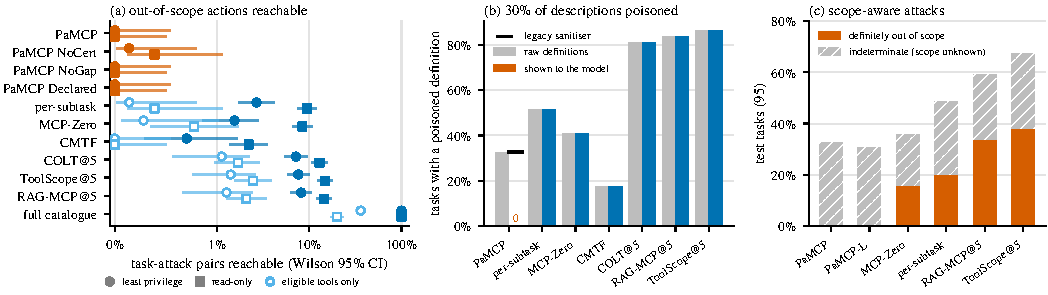
\includegraphics[width=\textwidth]{fig_sec_injection}
\caption{Security behaviour. (a) Task--attack pairs whose out-of-scope action the exposed toolkit can realise, as
published (filled) and restricted to eligible tools (open), under least-privilege and strict read-only policies
(symmetric log scale). (b) Tasks whose exposed definitions contain an injected instruction when 30\% of the
descriptions are poisoned: raw definitions of the toolkit against what the method shows the model. (c) Test tasks
with an attack that is definitely out of scope or of undecidable scope.}
\label{fig:ev-injection}
\end{figure*}

\emph{Reachable out-of-scope actions.} Under least-privilege policies none of the 712 task--attack pairs is
reachable through \pamcp{}'s toolkits, nor through NoGap, Declared or any component variant (Wilson upper bound
0.5\%), and one through NoCert, against 8.1\% for RAG-MCP, 7.6\% for ToolScope, 7.2\% for COLT, 2.7\% for
per-subtask retrieval, 1.5\% for MCP-Zero and 0.7\% for CMTF as published (Fig.~\ref{fig:ev-injection}a;
confirmatory F5 against per-subtask retrieval: $\Delta=-0.027$, $p_{\mathrm{Holm}}<0.001$). Under a strict
read-only policy the baselines reach 8.4--14.7\% and \pamcp{} stays at 0 of 775. Restricting the baselines to
eligible tools lowers them to at most 1.4\%: most of the protection comes from eligibility, which any retriever
can adopt. The scope-aware analysis qualifies this result (Fig.~\ref{fig:ev-injection}c): on the 95 test tasks no
\pamcp{} toolkit admits an attack that is definitely out of scope, against 15.8\% for MCP-Zero, 20.0\% for
per-subtask retrieval, 33.7\% for RAG-MCP and 37.9\% for ToolScope (H5, \pamcp{}-L against per-subtask retrieval:
$\Delta=-0.200$, 95\% CI $[-0.284, -0.126]$, $p_{\mathrm{Holm}}<0.001$), but 32.6\% of its toolkits admit an
attack whose scope the labels cannot decide. A write permitted by the policy is therefore not a proof that every
write is in scope; deciding it needs scoped effect labels that the benchmarks do not provide.

\emph{Poisoned metadata.} With 30\% of the descriptions poisoned, the raw definitions of \pamcp{}'s toolkits
contain an injected instruction in 32.6\% of the tasks, and those of the baselines in 17.4\% (CMTF) to 86.2\%
(ToolScope) (Fig.~\ref{fig:ev-injection}b). The aliased manifest, which shows the model only aliases, typed
arguments and the certificate, never shows one, in any of the three channels; the earlier sanitiser, which removed
descriptions but kept provider names and argument keys, would have shown one in as many tasks as the raw
definitions, through the tool name. Of \pamcp{}'s toolkits, 55.5\% contain a tool that returns remote content, an
indirect-injection channel, but none of them also allows an out-of-scope action, against 3.2--22.6\% for the
baselines.

\begin{table}[t]
\centering
\caption{Mechanism ablation on 155 tasks under least-privilege policies: the $2^3$ design over the gap (G),
provenance-sound eligibility (P) and set-level reasoning (S), and five components of the full configuration.
Reach: task--attack pairs whose out-of-scope action the toolkit can realise.}
\label{tab:ev-factorial}
\scriptsize
\setlength{\tabcolsep}{3pt}
\begin{tabular}{@{}cccrrrrr@{}}
\toprule
G & P & S & Recall & Tokens & Joint (\%) & Reach (\%) & Abst. (\%) \\
\midrule
-- & -- & -- & 0.270 & 297 & 53.5 & 1.1 & 0.0 \\
on & -- & -- & 0.239 & 208 & 55.5 & 0.4 & 0.0 \\
-- & on & -- & 0.295 & 316 & 58.1 & 0.1 & 0.0 \\
-- & -- & on & 0.223 & 221 & 52.9 & 0.1 & 16.1 \\
on & on & -- & 0.253 & 229 & 56.8 & 0.1 & 0.0 \\
on & -- & on & 0.230 & 189 & 54.8 & 0.0 & 6.5 \\
-- & on & on & 0.183 & 193 & 55.5 & 0.0 & 20.0 \\
on & on & on & 0.181 & 176 & 56.1 & 0.0 & 10.3 \\
\midrule
\multicolumn{3}{@{}l}{Full, no backward closure} & 0.181 & 173 & 53.5 & 0.0 & 12.3 \\
\multicolumn{3}{@{}l}{Full, flow along derivations} & 0.236 & 206 & 60.6 & 0.0 & 5.8 \\
\multicolumn{3}{@{}l}{Full, no relevance term} & 0.167 & 141 & 54.8 & 0.0 & 10.3 \\
\multicolumn{3}{@{}l}{Full, no utility floor} & 0.181 & 176 & 56.1 & 0.0 & 10.3 \\
\multicolumn{3}{@{}l}{Full, no refinement} & 0.179 & 175 & 55.5 & 0.0 & 11.0 \\
\bottomrule
\end{tabular}
\end{table}


\begin{figure*}[t]
\centering
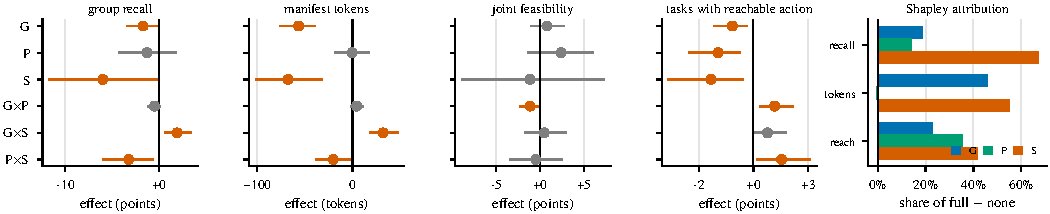
\includegraphics[width=\textwidth]{fig_sec_factorial}
\caption{Factorial analysis of the three mechanisms (155 tasks, least privilege): main effects and two-way
interactions with task-bootstrap 95\% CIs (orange: interval excludes zero), and the Shapley attribution of the
difference between the full configuration and the configuration without mechanisms.}
\label{fig:ev-factorial}
\end{figure*}

\emph{Mechanism contributions.} Table~\ref{tab:ev-factorial} and Fig.~\ref{fig:ev-factorial} separate the
mechanisms. Gap analysis and set-level reasoning each shrink the manifest (main effects $-56$ and $-67$ tokens,
both $p<0.001$); they are not additive (G$\times$S $+32$ tokens), and together they take the context from 297 to
176 tokens, with eligibility contributing nothing to size. All three mechanisms lower reachability (main effects
$-1.0$, $-1.6$ and $-1.9$ points; Shapley shares 23\%, 35\% and 42\%), from 5.2\% of the tasks without any mechanism
to none. Recall pays for the reduction: it falls from 0.270 to 0.181, mostly through set-level reasoning
($-6.0$ points, $p=0.042$) and its interaction with eligibility ($-3.2$, $p=0.018$). No mechanism changes joint
feasibility, which stays between 52.9\% and 58.1\% in every cell. The gap alone does not save significant tokens
once the other mechanisms are present (F6, full against NoGap: $\Delta=-16.7$, $p_{\mathrm{Holm}}=0.269$), but
it halves abstentions (10.3\% against 20.0\%), because goals the model can serve natively need no tool. Among the
components, removing backward closure raises abstentions to 12.3\%, propagating flow labels only along
derivations raises recall to 0.236 at the price of the order-independence of Property~1, and removing the
relevance term lowers recall to 0.167; the utility floor and refinement change little.

\emph{Interpretation.} Under the labelled, offline threat model, \pamcp{}'s toolkits leave no definite
out-of-scope action reachable and its manifest never carries an injected instruction, whereas retrieval
baselines expose both. The protection is shared between mechanisms: eligibility removes most reachable actions,
gap analysis and set-level reasoning shrink the exposed context and remove the rest, and the aliased manifest
closes the metadata channel. The same mechanisms cost recall, and none of them improves joint feasibility on its
own. Whether injected instructions are followed and executed by an agent, and whether runtime enforcement
blocks them, requires the execution environment discussed in Section~\ref{sec:ev-threats}.
